% !TEX root = ../main.tex

% = = = = = = = = = = = = = = = = = = = = = = = = = = = = = = = = = = = = = = = = = =

\section{Introductory Remarks}

Many stablecoins work like a hypothetical vending machine: Alice deposits two volatile coins (\eg a cryptocurrency like BTC or ETH) into the machine and it returns to her two new coins---a `black' coin that is stable and a `red' coin that is even more volatile in price than the original coins Alice put in. The machine cannot reduce overall price volatility, but it can push volatility from the black coin onto the red coin. 

Consider the following example of a stability mechanism that works similar to Clark et al.~\cite{CDM20}. An asset is chosen that is considered stable by definition (\eg the US dollar). The vending machine is implemented as a decentralize app (DApp; \aka smart contract) on a blockchain (\eg Ethereum). Alice deposits an amount of ETH worth \$1.50 USD into the DApp. The DApp references a trusted oracle service for the current ETH/USD exchange rate to enforce this. The DApp holds the ETH as a deposit for future redemption, and returns to Alice a red coin and a black coin (\eg as ERC-20 tokens). Alice can sell one or both coins. In the future, the owner of the black coin can redeem it for ETH from the DApp, and receives the equivalent of \$1.00 USD. This assumes the initial deposit of \$1.50 USD worth of ETH is still worth at least \$1.00 USD at redemption time---if not, the black coin owner receives all of the collateral. The red coin holder receives any remaining ETH after the black coin holder is paid.

The key idea is that the black coin will nearly always be worth the equivalent of \$1.00 USD. This is true when ETH/USD increases in value, stays the same, or declines moderately. Only if it declines significantly does the black coin start to experience volatility in price---it's redemption value will decrease at the same rate as ETH/USD itself. For the red coin, the redemption value increases and decreases as ETH/USD itself increases and decreases, however the gains and losses are amplified. This is an overview; we return to these details below.

\paragraph{Synthetic Assets.} The red-black coin primitive can be generalized to produce black coins that match the price of any financial asset, not just a currency like the USD, simply by changing the price that the oracle references. For example, a black coin for one share of the company Apple (APPL) would use an ETH/APPL price feed (possibly constructed by bridging ETH/USD and APPL/USD prices) and otherwise be exactly the same. These black coins are `synthetic assets' because they expose the holder to the price movements of the asset but do not afford the holder any other benefits of holding the financial instrument (\eg shareholder votes or dividends for equities; physical delivery for futures; or the ability to settle a loan, repo, or option contract on the asset). What a red coin represents this example is less natural than for a stablecoin: it is a bet that ETH will increase in price faster than APPL.

\paragraph{Relation to Dai.} Red-black coins are a primitive that has been used to build larger stablecoin systems like MakerDAO's currency \dai. In Maker, black coins are called \dai and a red coin is a \vault (\nee collateralized debt position or \cdp). However the system is immensely more complicated because it adds a number of features that the basic red-black coin primitive lacks: (1) interchangeability (fungibility) of red coins across multiple producers, (2) a liquidation process to incentive black coin holders to increase the collateralized ETH as ETH/USD declines or face an auction that automatically settles a red-black pair, and (3) fees to balance supply/demand of red coins with black coins that are adjustable through a distributed governance.
%Mentioning why we choose Dai to describe on the paper 
 %1. Dai has largest market cap between stable coins and synthetic assets
 %2. Due to space limitations we can't have more examples

%Somewhere we can put this:
%In this paper we are talking about some known financial instruments like Forward, %Futures, and options but we cannot describe them in detail because of space %limitations. For more detail the reader can use Options, futures and other %derivatives book by John C. Hull
\subsection{Contributions} In this paper, we study the red-black coin primitive to better understand its characteristics in isolation, which seems prudent before analyzing more complex systems. We use methods from quantitative finance to model how risky red and black coins are under different scenarios. We then examine the necessity of the extra infrastructure projects like MakerDao add to red-black coins---precisely what does the added complexity (\eg stability fees, liquidation, global shutdown, \etc) achieve and what are the design alternatives for the same functionality?

\subsection{Related Work} Several systemization of knowledge papers cover stablecoins~\cite{PHP+19,MSS20,CDM20}. Our notion of a red-black coin is inspired by the `indirectly-backed' classification from~\cite{CDM20}. Maker is considered a decentralized finance (DeFi) project and it (and other DeFi projects) has been studied from orthogonal angles including attacks/measurements on governance and oracles, attacks using flash loans, and modelling liquidity crises~\cite{GRB20,GPH+20,QZLG20,KMM20}. Our financial modelling uses the same methodology as~\cite{GPH+20}. Other projects built on the red-black primitive (for both stablecoins and synthetic assets) include Synthetix's sUSD, Kava's USDX, UMA, and BitUSD. 

% = = = = = = = = = = = = = = = = = = = = = = = = = = = = = = = = = = = = = = = = = =

\section{Financial Characteristics}

\begin{figure}[t]
\centering
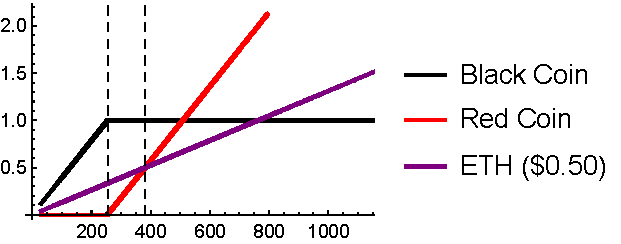
\includegraphics[width=0.6\columnwidth]{price1.pdf}
\caption{Redemption value in USD (y-axis) of a red coin, a black coin, and amounts of ETH equivalent to \$1 USD and \$0.50 USD as the price of ETH (x-axis) changes.\label{fig:price1}}
\end{figure}

In this section, we answer questions about the financial characteristics of the red-black primitive. Consider a black coin that targets \$1 USD when 1 ETH is \$381.56 USD, and the DApp holds 0.00393126 ETH (worth \$1.5 USD).  Assume no one intervenes when ETH/USD declines enough that black coins starts to lose value. Figure~\ref{fig:price1} shows how much a black coin is worth (y-axis) as the price of ETH varies (x-axis). The starting point (\$381.56 USD) is marked and if the price of ETH increases (rightward), the black coin is always worth \$1. If the value of ETH decreases (leftward), the black coin is still stable until the value of ETH hits \$254.37 (marked)---at this point, 0.00393126 ETH starts to become worth less than \$1 and the black coin `breaks the buck.'

Figure~\ref{fig:price1} also shows the redemption value of a red coin. When created, a red coin is redeemable for \$0.50 USD. A user with \$0.50 USD can choose between purchasing a red coin or purchasing ETH (also shown). In both cases, the user profits when ETH increases and loses when ETH decreases in price. However the slope of red coin is greater. This indicates it is a \emph{leveraged} position in ETH.  

% = = = = = = = = = = = = = = = = = = = = = = = = = = = = = = = = = = = = = = = = = =

\subsection{How much should you pay for a black coin?}

Consider a black coin that is purchased today when ETH is \$381.56 USD. How much will it be worth in 100 days? In most future worlds, the black coin will be worth \$1. In some future worlds, when ETH is worth less than \$254.37, the black coin breaks the buck, but even here, it takes a `haircut' on value as opposed to being worthless (\eg it can be redeemed for, say, \$0.90). 

\begin{figure}[t]
    \centering
        \subfloat[Price of ETH in USD (y-axis) over number of days (x-axis).]{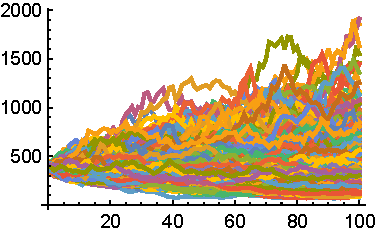
\includegraphics[width=0.45\columnwidth]{figures/mc.pdf}}
        \qquad
        \subfloat[Histogram of final price of ETH in USD (x-axis).]{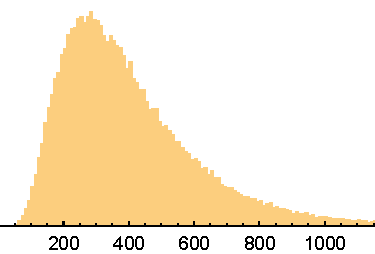
\includegraphics[width=0.45\columnwidth]{figures/histro.pdf}\label{fig:histro}}
    \caption{ETH/USD Monte Carlo simulation results. \label{fig:sim}}
\end{figure}

The expected value of a black coin can be estimated if we have a statistical model for ETH price movements. In finance, many statistical models have been proposed for many assets. For a first look, we use geometric Brownian motion (GBM), which underlies the Black-Scholes model for pricing options~\cite{BS73} and has been used for ETH in other work~\cite{GPH+20}. We omit the details of the model itself (covered in nearly every  financial textbook~\cite{Sey09}). We fit the model to the historical `closing' prices of ETH for 1000 days prior to 18 Sept 2020\footnote{CoinGecko API: \url{https://api.coingecko.com}} and obtain $\mu=0.000744754$ (an upward drift in price over time) and $\sigma=0.0524172$ (a measure of volatility). If we simulate the next 100 days using Monte Carlo, we obtain the results in Figure~\ref{fig:sim}. For the parameters of this example, the expected value of the black coin \$0.94 USD. Our model can be adjusted for the initial price, over-collateralization ratio (see ~\ref{sec:redchar}), and days until redemption. It is available in Python and Mathematica.\footnote{GitHub: URL omitted for anonymity.} 

As shown in Figure~\ref{fig:sim}\subref{fig:histro}, the expected return is log-normal. When we model 200 days, instead of 100, the variance increases, adding more occurrences of black coins slipping below \$1 but slipping along a gentler curve. The net effect is a decrease in value. The expected redemption value of our black coin is \$0.94 USD after 100 days, \$0.85 USD after 200 days, and \$0.80 after 1 year. 

% = = = = = = = = = = = = = = = = = = = = = = = = = = = = = = = = = = = = = = = = = =

\subsection{Why would you want a red coin?}
\label{sec:redchar}

While a stablecoin has utility to the holder, it is less clear what the utility of a red coin is. Margin trading is popular in traditional financial markets so speculators can obtain a leveraged position. \textcolor{red}{In margin trading, the investor borrows some money from the broker to buy more stocks than she can get. However, she promises to pay back the loan after closing the position. Leverage is the ratio between the amount of money she has and the amount of money she can trade after borrowing.} \textcolor{red}{A black coin holder pays \$1 at the first day and expect to recieve \$1 in future and it is like lending this money to the red coin holder}. A red coin holder, acquires the profits and losses from both the black coin's ETH (initial redemption value of \$1) and the remaining over-collaterized ETH (initial redemption value of \$0.50). Investing in a red coin is equivalent to investing \$0.50 along with a borrowed $2\times\$0.50$ in ETH (\ie 3:1 leverage). 

If the over-collateralization ratio is decreased from 1.50 to 1.10, then leverage for the red coin increases to 11:1. However the black coins becomes riskier and its 100-day expected value drops from \$0.94 to \$0.86. For a \$2.00 collateralization, red coin leverage is 2:1, and black coin value is \$0.98. 

\begin{figure}[t]
\centering
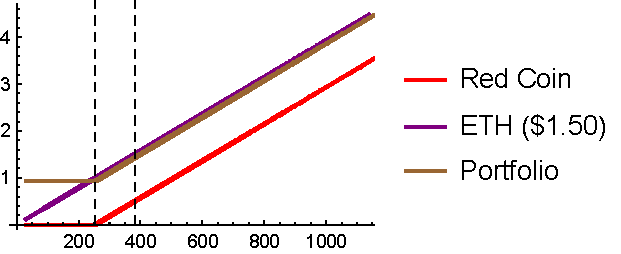
\includegraphics[width=0.6\columnwidth]{price2.pdf}
\caption{Redemption value in USD (y-axis) of a red coin, ETH equivalent to \$1.50 USD, and a portfolio of a red coin and \$1.\label{fig:price2}}
\end{figure}

Speculators seek out red coins. Consider a trader that holds ETH (assume for now with 0\% interest) and does not want leverage---she seemingly has no interest in red (or black) coins. In scenario A, she holds \$1.50 worth of ETH. In B, she takes her \$1.50 worth of ETH, issues and sells a black coin (\eg for \$0.94 USD), and holds the red coin. She actually has a small portfolio of a red coin and close to \$1 USD. The redemption value of A and B are depicted in Figure~\ref{fig:price2}, along with the red coin by itself. The portfolio is actually an attractive investment---she has `insurance' against catastrophic loss during a devaluation of ETH for a small fixed `fee'---the \$0.06 USD difference between what she recieved for the black coin (\$0.94) and what the DApp pays out to the black coin holder (\$1.00). Additionally, she produced a stable black coin, which has external benefit to the decentralized economy. 

Finally, we can revise our assumption and assume she can earn interest on ETH (through advances in DeFi). However this does not change the point as decentralized lending (\eg Compound )can allow red coins to earn interest with the same mechanism used for ETH, and the USD can also earn a return.%reference for compound

% = = = = = = = = = = = = = = = = = = = = = = = = = = = = = = = = = = = = = = = = = =

\section{Extending Red-Black Coins}

Red-black coins are primitives. Other aspects of their design need to be determined before they could actually be deployed. Design decisions include the maturity/redemption policy, how to make black and red coins fungible, and interventions to prevent the black coin from breaking the buck. One set of decisions lead to a design like MakerDao's \dai, however there are other decisions that could result in very different stablecoins. The purpose of this section to emphasize that \dai is one set of reasonable decisions but there are many alternative designs that have not been (to our knowledge) explored.

% = = = = = = = = = = = = = = = = = = = = = = = = = = = = = = = = = = = = = = = = = =

\subsection{Fungibility}

Assume Alice creates a red/black coin, selling the red coin to Bob. Later, Carol creates a red/black coin, selling the red coin to David. Alice's black coin is not identical to Bob's black coin. Because they were created at different times, the ETH/USD exchange rate is different, and thus the  amount of collateral in ETH in the DApp will be different. The more collateral, the more a black coin is worth (recall Section~\ref{sec:redchar}). Such coins are not interchangeable or \textit{fungible} which adds effort to valuation and exchange. 

One design option is to \textbf{(1) forgo fungibility} and have each coin pair be its own individual contract between two counter-parties. This is principle of forward contracts. A second option is to \textbf{(2) pool the collateral} of the red coins so that each black coin is a claim against the pool. This is how \dai works. A pool can be unfair: if Alice obtains a red coin before an ETH/USD price bubble, she is not exposed to the bubble bursting (assuming it returns to the pre-bubble price). However in a pool, all the red coins issues during the rising bubble are backed by significantly less collateral and when bubble bursts, the pool becomes under-collateralized. The losses are democratized to all red coin holders including Alice. 

% = = = = = = = = = = = = = = = = = = = = = = = = = = = = = = = = = = = = = = = = = =

\subsection{Redemption}

A policy for redeeming the collateralized ETH is the first design decision. Note that the DApp can autonomously distribute the collateral without the participation of the red or black coin holder, however someone needs to trigger a function call against the DApp to finalize the process.

 Red-black coins could \textbf{(1) mature on a pre-specified date} (\eg the first day of a specified month). At any given time, red/black coins in circulation would have one of a few different expiration dates, while still allowing some degree of fungibility. Coin holders would shorten or extend their coins by trading for a coin with a different maturity date. This is precisely how futures mature, and yTokens are based on the same principle~\cite{RoNi20}. After maturity, the DApp would lock all transfer functions and only allow withdrawal by the coin holders. The first to ask for a withdrawal would trigger the DApp to look up the ETH/USD price as of the maturity date and split the collateral accordingly. 

Alternatively, red-black coins could be redeemed at any time \textbf{(2) on demand by the black coin holder}, or \textbf{(3) red coin holder}, \textbf{(4) either}, or \textbf{(5) both}. Options (in the US style) work on the principal of (2) or (3), and price of a coin (\cf derivative~\cite{Sey09}) that is redeemable on-demand strengthens. Allowing either to redeem is unlike anything we could find in traditional finance---we speculate it would add uncertainty without any clear gain. Requiring both to agree to redemption is not actually an agreement \textit{per se}, the idea is a black coin holder would purchase a fungible red coin (or conversely, a fungible black coin for a red coin holder) and redeem the collateral on-demand. This is how \dai works, using fungible black coins and non-fungible red coins. 

% = = = = = = = = = = = = = = = = = = = = = = = = = = = = = = = = = = = = = = = = = = = = = = = = = =


\subsection{Under-collateralization}

When the ETH/USD exchange rate drops enough that under-collateralization is possible, the system could \textbf{(1) do nothing} and let the black coin holder price the risk of this into the coin, or the design could attempt further mitigation. In traditional financial markets, exchanges attempt to quickly liquidate a trader's losing position when the trading account balance dips below a threshold. Similarly, the DApp could require red coin holders to top-up their collateral and \textbf{(2) liquidate} it (\eg sell it by auction for black coins) if they do not. When collateral is pooled, this is crucial because under-collateralized red coins hurt all black coin holders. When collateral is not pooled, liquidation is useless for black coin holders because both ETH and black coins decrease in value at the same rate (recall Figure~\ref{fig:price1}) so it is simpler to do nothing.

Liquidation does not incentivize topped-up collateral unless if it is accompanied by a \textbf{(3) punishment} (otherwise black coin holders might try to buy their liquidated assets from themselves at a discount). Beyond charging a fee, a stablecoin system might also withhold rewards (some systems used a secondary token for providing governance and providing rewards) or block red transfers until collateral is restored. In traditional financial markets, it is also the case that a trader's margin is inadequate to settle their account, they are still legally liable for the difference. A stablecoin accompanied by a \textbf{(4) reputation system} could mandate that black coin holders settle any obligation, however this increase the bound on how much a black coin holder can lose. A different approach is to obtain \textbf{(5) insurance} or financial coverage for the event of a decline in ETH/USD. This could be actual insurance, whether decentralized or through a traditional brokerage, or an offsetting financial investment that hedges the currency exchange risk.


The last approach is \textbf{(6) bail out} any loses through sales of a secondary token. This was used recently by MakerDao for \dai holders when its normal procedures of (2) and (3) were not adequate for dealing with a sharp, unexpected decline in the price of ETH on 12 Mar 2020 (`black Thursday'). While the auction was successful and recollateralized the pool, it cannot be generally guaranteed that minting new tokens will always be adequate for offsetting any debt. This event also exposed the lack of understanding and underestimation of risk by many vault (\ie red coin) holders who faced losses under (3), and raises the question of whether a system should be designed that is more forgiving to red coin holders in turbulent markets, especially since their financial position enables the issuance of a stablecoin. 


% = = = = = = = = = = = = = = = = = = = = = = = = = = = = = = = = = = = = = = = = = = = = = = = = = =


\subsection{Autonomy} 

The red-black coin primitive is entirely autonomous, which can be instantiated in a DApp and operate without human intervention. While the core primitive provides price-stability, traders who are time-sensitive may forgo obtaining a good price in order to trade quickly. This particularly is influential for stablecoins which provide a low-friction avenue in and out of speculative positions on the price of ETH. Since red and black coins are issued in the same proportion, supply/demand imbalances between them adds volatility to the black coin price. This could potentially be addressed in the design. 

A non-interventionist approach would let the red and black coin price \textbf{(1) float freely}. This avoids adding complexity to the design, and a design goal might be a system traders can easily understand and grasp the risk of. An alternative is to further stabilize prices by \textbf{(2) setting rates and fees} at various points in the system. For example, if black coin holders can redeem at any time, a fee could be charged to the black coin holder and paid to the red coin holder. If redemption requires both a red and black coin, the fee could be collected by the DApp. This principle is used by central banks for targeting interest rates, and is used in MakerDAO to control the spot market for \dai. It is a struggle to set fees in the context of a decentralized and autonomous organization---while allowing decisions to be voted on is a first step, it does not guarantee that token holders are independent, informed, and not unduly influenced by the `expert' recommendations. 

% = = = = = = = = = = = = = = = = = = = = = = = = = = = = = = = = = = = = = = = = = = = = = = = = = =
% = = = = = = = = = = = = = = = = = = = = = = = = = = = = = = = = = = = = = = = = = = = = = = = = = =
% = = = = = = = = = = = = = = = = = = = = = = = = = = = = = = = = = = = = = = = = = = = = = = = = = =

\section{Concluding Remarks}

In this paper, we distil complex stablecoin systems into one of their core primitives, the red-black coin and provide a detailed study of its characteristics and possible extensions. It would be useful to have research results on the most suitable financial model for the ETH/USD price rate (\eg drift-diffusion models instead of simple GBM) for us to use in work like this paper. Future work could also examine the benefits of building a \dai alternative, still based on red-black coins but using different design parameters. Two examples that seem interesting are: (a) a simpler system that reduces the amount of intervention, and (b) . Finally, while our paper answer the question of how much you should pay for a black coin, the analysis is much more complicated for \dai --- with pooled collateral, liquidation, and bailouts, \dai is less risky than a simple black coin but the risk that these countermeasures systemically fail is not zero.

